\documentclass[11pt,a4paper]{article}
\usepackage{fontspec}
\usepackage{polyglossia}
\setdefaultlanguage{polish}
\usepackage{geometry}
\usepackage{graphicx}
\usepackage{booktabs}
\usepackage{hyperref}
\usepackage{subcaption}
\usepackage{amsmath}

\geometry{margin=2.5cm}
\graphicspath{{../results/compare/local/}{../results/local/viz_beta1/rep1/}{../results/local/viz_beta4/rep1/}}

\title{Lab07 --- Równoległy Metropolis dla modelu Isinga (2D, MPI)}
\author{Programowanie równoległe --- UMISI}
\date{\today}

\begin{document}
\maketitle

\section{Wprowadzenie}
Model Isinga opisuje układ spinów $\sigma_{ij}\in\{-1,+1\}$ na sieci kwadratowej
z sąsiedztwem von Neumanna. Hamiltonian z $J=1$, $h=0$:
\[
H = -\sum_{\langle ij\rangle} \sigma_i \sigma_j .
\]
Symulacja przebiegu Monte Carlo realizuje schemat Metropolisa: w każdej próbie
losowany jest spin; obrót akceptowany, gdy $\Delta E\le 0$, w przeciwnym razie
z prawdopodobieństwem $\min(1,e^{-\beta\Delta E})$.

\section{Implementacja równoległa}
\subsection{Dekompozycja}
Siatka $L\times L$ dzielona jest na $P$ poziomych pasów wysokości $h=L/P$.
Każdy proces przechowuje tablicę $(h+2)\times L$ z jednym wierszem halo u góry i u dołu.
Warunki periodyczne w kierunku $y$ realizuje pierścień MPI; w $x$ --- lokalnie.

\subsection{Spójność losowań}
Generator indeksów spinów inicjalizowany tym samym \texttt{seed} na wszystkich
procesach (w każdym MCS osobno). Liczby losowe w akceptacji generowane niezależnie
(\texttt{SeedSequence.spawn}).

\subsection{Synchronizacja}
\textbf{border:} wymiana halo przy każdej próbie spinu brzegowego (wiersz $1$ lub $h$).
\textbf{smart} (Barkema, MacFarland): kolumnowe flagi nieaktualnego halo; komunikacja
tylko gdy wylosowany spin brzegowy wymaga aktualnego sąsiada.

Pętle flipów w \texttt{Numba @njit}; komunikacja \texttt{Sendrecv} w Pythonie.

\subsection{PCAM}
\begin{itemize}
  \item \textbf{P:} podział na pasma poziome.
  \item \textbf{C:} wymiana wierszy halo; brak komunikacji między flipami wewnętrznymi.
  \item \textbf{A:} gromadzenie $E$, $M$ przez \texttt{Allreduce}; układ przez \texttt{Gather}.
  \item \textbf{M:} 1 proces $\leftrightarrow$ 1 pas; stała liczba procesów na węźle.
\end{itemize}

\section{Wyniki wizualizacji ($\beta=1$, $\beta=4$)}
\begin{figure}[ht]
  \centering
  \IfFileExists{lattice.png}{%
    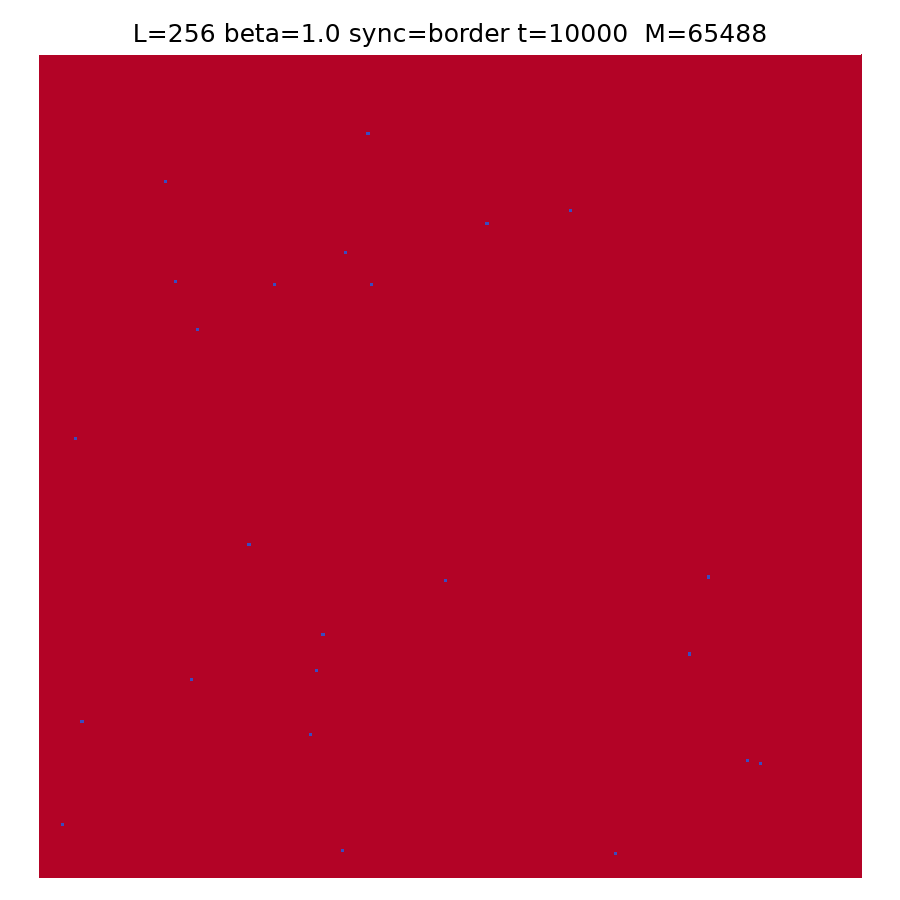
\includegraphics[width=0.45\linewidth]{lattice.png}}{}
  \IfFileExists{../results/local/viz_beta4/rep1/lattice.png}{%
    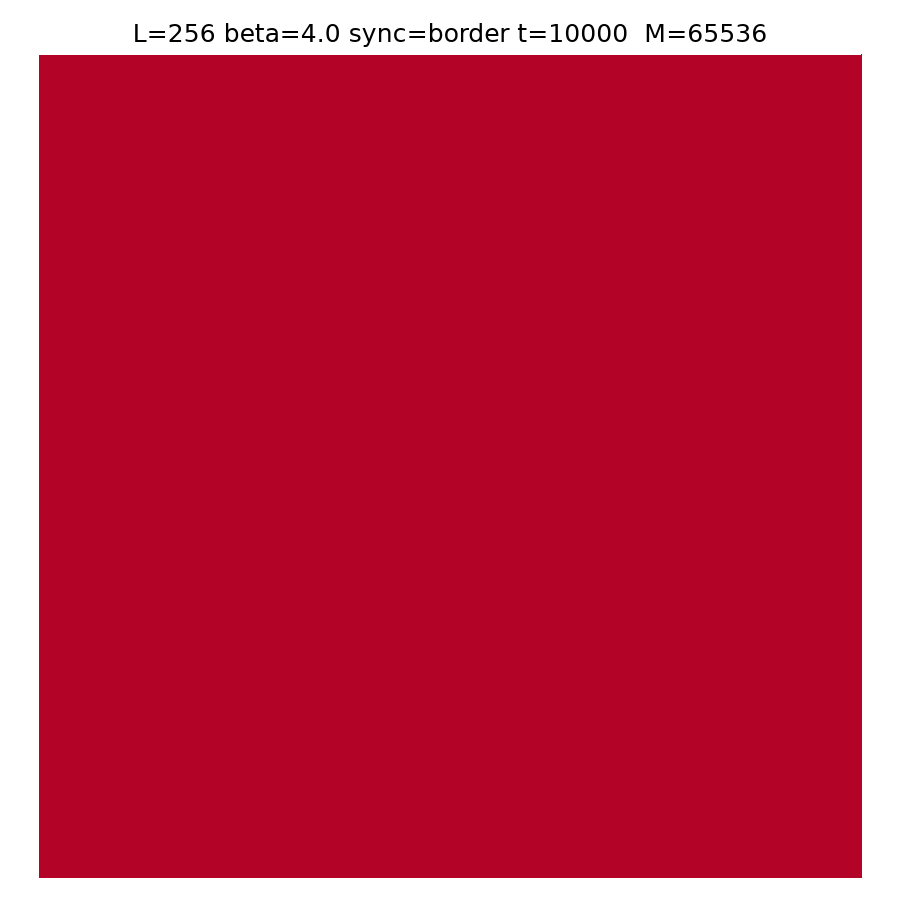
\includegraphics[width=0.45\linewidth]{../results/local/viz_beta4/rep1/lattice.png}}{}
  \caption{Stan końcowy po $t=10\,000$ MCS ($L=256$, $P=4$, \texttt{border}).}
\end{figure}

\section{Metryki wydajności}
Dla platformy \texttt{local} i siatki $L$:
\[
S = \frac{T(1)}{T(P)}, \quad E = \frac{S}{P}, \quad
f = \frac{1/S - 1/P}{1 - 1/P}.
\]

\begin{figure}[ht]
  \centering
  \IfFileExists{../results/compare/local/speedup_vs_p_L960.png}{%
    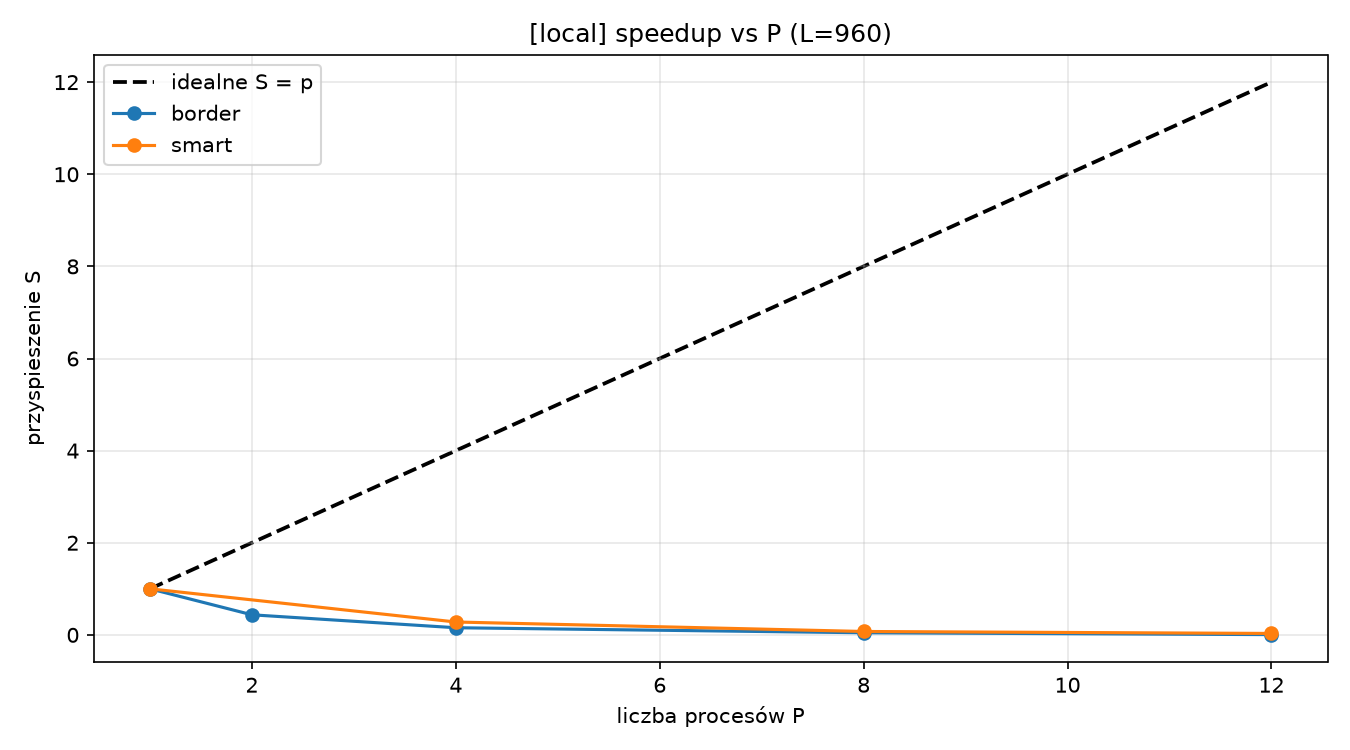
\includegraphics[width=0.9\linewidth]{speedup_vs_p_L960.png}}{%
    \textit{Uruchom \texttt{local/sweep.sh}, potem \texttt{report/build.sh}.}}
  \caption{Przyspieszenie $S$ vs.\ liczba procesów.}
\end{figure}

\IfFileExists{../results/compare/tex/metrics_local_L960.tex}{%
  \begin{tabular}{lrrrrr}
\toprule
sync & $P$ & $T$ [s] & $S$ & $E$ & $f$ \\
\midrule
border & 1 & 5.2578 & 1.000 & 1.000 & --- \\
border & 2 & 12.0637 & 0.436 & 0.218 & 3.589 \\
border & 4 & 33.9053 & 0.155 & 0.039 & 8.265 \\
border & 8 & 114.0383 & 0.046 & 0.006 & 24.645 \\
border & 12 & 931.2153 & 0.006 & 0.000 & 193.121 \\
smart & 1 & 3.2181 & 1.000 & 1.000 & --- \\
smart & 4 & 11.5192 & 0.279 & 0.070 & 4.439 \\
smart & 8 & 43.6092 & 0.074 & 0.009 & 15.344 \\
smart & 12 & 102.9489 & 0.031 & 0.003 & 34.808 \\
\bottomrule
\end{tabular}
}{}

\section{Wnioski}
Tryb \texttt{smart} zmniejsza liczbę synchronizacji na MCS w stosunku do
\texttt{border}, co poprawia $S$ przy dużym $P$. Przy małym $L/P$ dominuje narzut MPI.
Dla $\beta=4$ układ ferromagnetyczny --- dominacja jednej fazy; dla $\beta=1$ --- stan
paramagnetyczny (duża magnetyzacja szczegółowa bliska zera w średniej).

\end{document}